%\documentclass[en,undergrad]{GTUThesis}
\documentclass[tr,graduate]{GTUThesis}

%% Fill in these
\GTUAuthor{Usama Derbashi}
\GTUTitle{Discrete Fourier Transformation}
\GTUFaculty{Faculty of Engineering}
\GTUDepartment{Computer Engineering}
\GTUProject{Bachelor's Thesis}
\GTUSupervisor{Assoc. Prof. Alp Arslan Bayrakci}
\GTUYear{2022}
%% Jury is comma separated
\GTUJury{Prof. Erchan Aptoula, M.Sc Melike Ilteralp}
\GTUDecreeNo{120/5658}
\GTUDecreeDate{14/06/2021}
\GTUDefenceDate{04/07/2022}

\usepackage{lipsum}

\begin{document}

\GTUMakeFront

\chapter{Usage}

\section{Project Structure}

In order to use the project more efficiently I thought an explanation of the structure of the project would be a good place to start to further the understanding of the different elements of the project. \Cref{fig:struct} shows the structure.

\begin{figure}
    \centering
    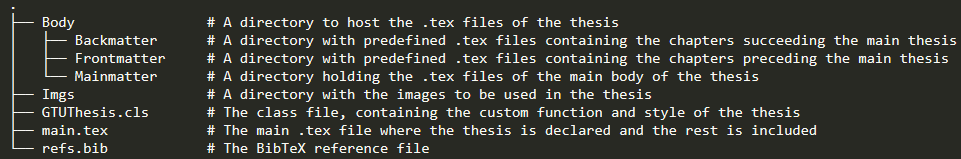
\includegraphics[width=\linewidth]{struct}
    \caption{The structure of the project, if too small please refer to the Github repo\cite{github}}
    \label{fig:struct}
\end{figure}


\section{Backmatter and Frontmatter}

As mentioned in the structure, these directories (\texttt{./Body/Backmatter} and \texttt{./Body/Frontmatter}) contain \texttt{.tex} files with the chapters preceding and succeeding the main body of the thesis, like abstract, list of acronyms, and appendices. The comments in the files themselves indicate where and what to write. Please don't edit the areas not meant to be edited.

\section{Mainmatter}\label{sec:mainmatter}

The \texttt{./Body/Mainmatter} directory is to house the \texttt{.tex} files of the main body of the thesis to be later included in the \texttt{./main.tex} (see \Cref{sec:maintex}). They can be named anything and organised within the directory in any way deemed fit. The example has two files (\texttt{C1.tex} and \texttt{C2.tex}) demonstrating a way of using the files, but it can be used in any other way, name or convention deemed appropriate by the user.

\section{Imgs and refs.bib}

As mentioned in the structure, \texttt{./Imgs} is a directory to house the images to be used in the figures of the thesis. The files in the directory could be further organised into subdirectories, but the file \texttt{./Imgs/gtu\_logo.jpg} to stay in its place.

As for \texttt{refs.bib}, this is a BibTeX file to be filled in with the references to be used for the thesis. (copied from the publisher or scholar.google.com)

\section{GTUThesis.cls}\label{sec:cls}

This is the file containing the custom functions and style of the GTU thesis. See \Cref{ch:class} for the documentation. \textbf{\textit{DO NOT}} modify this file unless you know what you're doing and sure about the changes you want to do.

\section{main.tex}\label{sec:maintex}

This is the main \texttt{.tex} file where the user firstly declares the document class as \texttt{GTUThesis} and then fills in the GTU-fields, followed by the used packages, and then starts the document environment, where they are expected to call the \texttt{GTUMakeFront} and \texttt{GTUMakeBack} functions respectively right after the start and before the end of the document environment. See \Cref{ch:class} for the documentation.

Between the \texttt{GTUMakeFront} and \texttt{GTUMakeBack} functions the user can include the files of the Main matter (recommended, see \Cref{sec:mainmatter}) using the include function as follows:

	\texttt{~~~~\textbackslash include\{./Body/Mainmatter/FILE.tex\}}

or write their thesis in the way they see fitting.

\section{Important Note}

\textbf{\textit{DO NOT}} delete, rename, or move the following files or directories because their paths are hard-coded:
\begin{itemize}
    \item \texttt{./Body}
    \item \texttt{./Body/Backmatter}
    \item \texttt{./Body/Backmatter/Appendices.tex}
    \item \texttt{./Body/Backmatter/CV.tex}
    \item \texttt{./Body/Frontmatter}
    \item \texttt{./Body/Frontmatter/Abstract.tex}
    \item \texttt{./Body/Frontmatter/Acknowledgement.tex}
    \item \texttt{./Body/Frontmatter/ListOfAcro.tex}
    \item \texttt{./Body/Frontmatter/Ozet.tex}
    \item \texttt{./Imgs}
    \item \texttt{./Imgs/gtu\_logo.jpg}
    \item \texttt{./GTUThesis.cls}
    \item \texttt{./refs.bib}
\end{itemize}
\chapter{GTUThesis Class} \label{ch:class}

\texttt{GTUThesis.cls} (see \Cref{sec:cls}) is the star of the show here, where the style of the thesis of GTU is defined. The user is expected to use some functions, and the demo \texttt{main.tex} shows how it is used. But for the sake of completion,  here is the documentation for the functions which the user is expected to call in their main.

\section{Declare Class}\label{sec:declare}

	\texttt{~~~~\textbackslash documentclass[lang,degree]\{GTUThesis\}}

The \texttt{lang} and \texttt{degree} options are set to set the language of the thesis (including titles and predefined text), and the degree which mainly changes some slight things in the Frontmatter. \texttt{lang} can take either \texttt{en} or \texttt{tr} with the former being the default, and \texttt{degree} takes either \texttt{undergrad} or \texttt{graduate} with the latter being the default.

\section{GTU Fields}

These are the fields required to be filled in at the beginning of the documents, they all take one argument in the following matter

	\texttt{~~~~\textbackslash GTUField\{argument\}}

and they are the following.

\begin{table}
    \caption{GTU-fields and their arguments}
    \label{tab:fields}
    \centering
    \begin{tabular}{|l|l|l|}
        \hline
        \textbf{GTU Field} & \textbf{Taken Argument} \\
        \hline
        GTUAuthor & Name of the author of the thesis (student)\\
        GTUTitle & The title of the thesis\\
        GTUFaculty & The faculty or institute of the author\\
        GTUDepartment & The department of the author\\
        GTUProject & The project the author is working on (ex. PhD thesis)\\
        GTUSupervisor & Name of the supervisor\\
        GTUYear & The year of the publication of the thesis\\
        GTUJury & Names of the jury for the thesis (comma separated) \\
        GTUDefenceDate & The date when the author presents the project to the jury\\
        GTUDecreeNo & The decree number of the jury formation (only graduate)\\
        GTUDecreeDate & The above decree's date (only graduate)\\
        \hline
    \end{tabular}
\end{table}


\section{GTU Make}

These are two functions which produce the front-matter and the back-matter of the thesis.

	\texttt{\textbackslash GTUMakeFront}

The function above produces the front-matter including the cover, the lists of content, figures, tables, and acronyms etc. in the correct order and in the correct format for the declared class's arguments (see \Cref{sec:declare} for more).

	\texttt{\textbackslash GTUMakeBack\{arg\}}

The function above produces the back-matter including the bibliography, and the optional CV and appendices. \texttt{arg} is a string that takes in the optional sections which the user wants to add comma separated (\texttt{cv} for the CV and \texttt{ap} for the appendices). If the user still doesn't want any optional sections, they still have to add the empty \texttt{\{\}} since the function waits for an argument which can be an empty string. So, the valid uses of the function are 

	\texttt{\textbackslash GTUMakeBack\{\} \% for only bibliography}
	
	\texttt{\textbackslash GTUMakeBack\{cv\} \% for bibliography and CV}
	
	\texttt{\textbackslash GTUMakeBack\{ap\} \% for bibliography and appendices}
	
	\texttt{\textbackslash GTUMakeBack\{cv,ap\} \% for bibliography, CV, and appendices}

\section{A Section to catch some other things}


Let $X_1, X_2, \ldots, X_n$ be a sequence of independent and identically distributed random variables with $\text{E}[X_i] = \mu$ and $\text{Var}[X_i] = \sigma^2 < \infty$, and let
\begin{equation}
    S_n = \frac{X_1 + X_2 + \cdots + X_n}{n}
      = \frac{1}{n}\sum_{i}^{n} X_i
\end{equation}
denote their mean. Then as $n$ approaches infinity, the random variables $\sqrt{n}(S_n - \mu)$ converge in distribution to a normal $\mathcal{N}(0, \sigma^2)$.

\begin{quote}
    \lipsum[10] \footnote{The text in this quote was created with \texttt{lipsum} package}
\end{quote}

% add cv or ap (comma separated) for CV or appendices if required
% they are optional arguments, otherwise leave {}  
\GTUMakeBack{cv, ap}

\end{document}